\documentclass[12pt,a4paper]{article}
\usepackage[utf8]{inputenc}
\usepackage{amsmath, amssymb}
\usepackage{graphicx}
\usepackage{geometry}
\usepackage{float}
\usepackage{booktabs}
\usepackage{caption}
\usepackage{circuitikz}
\geometry{a4paper, margin=1in}

\title{\textbf{08. Differential Amplifier using transistor - CMRR}}
\author{Yamulapalli Nandu Navadeep \\ Roll Number: IMS24267}
\date{Date of Experiment: 05/08/2026 \\ Date of Submission: 25/08/2026}

\begin{document}

\maketitle

\section{Aim of the Experiment}
To design a differential amplifier using transistors and to find out the Common Mode Rejection Ratio (CMRR).

\section{Theory}
A differential amplifier is a closed loop amplifier circuit which amplifies the difference between two signals. Such a circuit is very useful in instrumentation systems. Differential amplifiers have a high common mode rejection ratio (CMRR) and high input impedance.

The circuit consists of two identical transistors (Q1 and Q2) with their emitters coupled together. The collectors are connected to the main supply $V_{CC}$ through collector resistors $R_C$. The power supplies $V_{CC}$ and $-V_{EE}$ have the same magnitude.

The output voltage $V_o$ is given by:
$$V_o = A_d(V_{in1} - V_{in2})$$
Where $A_d$ is the differential gain, and $V_{in1}, V_{in2}$ are the input voltages.

When $V_{in1} = V_{in2}$, the output should ideally be zero. That is, a differential amplifier suppresses common mode signals.

\subsection{Differential Mode Gain ($A_d$)}
The amplification can be driven differentially by taking the output between the collector of Q1 and Q2. The differential mode gain is calculated as:
$$A_d = \frac{V_{out}}{V_{in1} - V_{in2}}$$

\subsection{Common Mode Gain ($A_c$)}
Common mode gain represents the gain of the differential amplifier when the same input is fed to both base terminals. The expected output will be very small, ideally zero.
$$A_c = \frac{V_{out}}{V_{in}}$$

\subsection{Common Mode Rejection Ratio (CMRR)}
The ability of a differential amplifier to reject common mode signals is called Common Mode Rejection Ratio (CMRR). It is defined as the ratio of differential mode gain to common mode gain.
$$CMRR = \left| \frac{A_d}{A_c} \right|$$
Usually, CMRR is expressed in decibels (dB):
$$CMRR_{dB} = 20 \log_{10}(CMRR)$$

\section{Procedure}
\begin{enumerate}
    \item \textbf{Design of the Circuit:} Calculate the values of $R_E$ and $R_C$ based on the given $V_{CC}$, $V_{EE}$, and desired $I_E$ and $V_{CE}$. 
    \item Connect the two transistors with emitters coupled and connect the calculated resistors.
    \item \textbf{Differential Mode:} Apply a known voltage to the first base ($V_{in1}$) and another voltage to the second base ($V_{in2}$). Measure the output voltage across the collectors. Calculate the differential gain $A_d$.
    \item \textbf{Common Mode:} Apply the same input signal ($V_{in}$) to both bases simultaneously. Measure the output voltage. Calculate the common mode gain $A_c$. Repeat for multiple input voltages.
    \item Calculate the CMRR and express it in decibels.
\end{enumerate}

\section{Circuit Diagrams}

\subsection{Differential Mode Circuit}
\begin{figure}[H]
\centering
\begin{circuitikz}[scale=0.8, transform shape]
    \draw (0,0) node[npn] (Q1) {Q1};
    \draw (4,0) node[npn, xscale=-1] (Q2) {\scalebox{-1}[1]{Q2}};
    
    % Emitter connection
    \draw (Q1.E) -- (Q2.E);
    \draw (2,-0.75) to[R, l=$R_E$] (2,-3) node[vee] {$-V_{EE}$};
    \draw (2,-0.75) -- (2,-0.75|-Q1.E);

    % Collector connection
    \draw (Q1.C) to[R, l=$R_C$] ++(0,2.5) coordinate (VCC1);
    \draw (Q2.C) to[R, l_=$R_C$] ++(0,2.5) coordinate (VCC2);
    \draw (VCC1) -- (VCC2);
    \draw (2, 3.25) -- (2, 4) node[vcc] {$+V_{CC}$};
    
    % Inputs
    \draw (Q1.B) to[R, l=$R_B$] ++(-2,0) to[sV, l=$V_{in1}$] ++(0,-2) node[ground]{};
    \draw (Q2.B) to[R, l_=$R_B$] ++(2,0) to[sV, l_=$V_{in2}$] ++(0,-2) node[ground]{};
    
    % Output
    \draw (Q1.C) to[short, *-o] ++(1,0) coordinate (out1);
    \draw (Q2.C) to[short, *-o] ++(-1,0) coordinate (out2);
    \draw (2, 1) node {$V_{out}$};
    \draw (3, 1.25) node {};
\end{circuitikz}
\caption{Differential Amplifier in Differential Mode}
\end{figure}

\subsection{Common Mode Circuit}
\begin{figure}[H]
\centering
\begin{circuitikz}[scale=0.8, transform shape]
    \draw (0,0) node[npn] (Q1) {Q1};
    \draw (4,0) node[npn, xscale=-1] (Q2) {\scalebox{-1}[1]{Q2}};
    
    % Emitter connection
    \draw (Q1.E) -- (Q2.E);
    \draw (2,-0.75) to[R, l=$R_E$] (2,-4) node[vee] {$-V_{EE}$};
    \draw (2,-0.75) -- (2,-0.75|-Q1.E);

    % Collector connection
    \draw (Q1.C) to[R, l=$R_C$] ++(0,2.5) coordinate (VCC1);
    \draw (Q2.C) to[R, l_=$R_C$] ++(0,2.5) coordinate (VCC2);
    \draw (VCC1) -- (VCC2);
    \draw (2, 3.3) -- (2, 4) node[vcc] {$+V_{CC}$};
    
    % Inputs connected together
    \draw (Q1.B) to[R, l=$R_B$] ++(-2,0) coordinate (B1);
    \draw (Q2.B) to[R, l_=$R_B$] ++(2,0) coordinate (B2);
    \draw (B1) -- ++(0,-1.5) coordinate (B1low);
    \draw (B2) -- ++(0,-1.5) coordinate (B2low);
    \draw (B1low) -- (B2low);
    \draw (B1low) to[sV, l=$V_{in}$] ++(0,-1.5) node[ground]{};
    
    % Output
    \draw (Q1.C) to[short, *-o] ++(1,0) coordinate (out1);
    \draw (Q2.C) to[short, *-o] ++(-1,0) coordinate (out2);
    \draw (2, 1.25) node {$V_{out}$};
\end{circuitikz}
\caption{Differential Amplifier in Common Mode}
\end{figure}

\section{Calculations}

Given parameters:
\begin{itemize}
    \item $V_{CC} = 15$ V, $V_{EE} = -15$ V
    \item $V_{CE} \approx 7.5$ V
    \item $I_E = 1$ mA ($1 \times 10^{-3}$ A)
    \item $V_{BE} = 0.7$ V
\end{itemize}

\subsection{Design of Emitter Resistor ($R_E$)}
The emitter resistor determines the emitter current of Q1 and Q2.
$$R_E = \frac{|V_{EE}| - V_{BE}}{2I_E}$$
$$R_E = \frac{15 - 0.7}{2(1 \times 10^{-3})} = \frac{14.3}{2 \times 10^{-3}} = 7.15 \text{ k}\Omega$$

\subsection{Design of Collector Resistor ($R_C$)}
Assuming $I_C \approx I_E = 1.05$ mA for real-life adjustment:
$$V_C = V_{CC} - (I_C \times R_C)$$
$$7.5 = 15 - (1.05 \times 10^{-3} \times R_C)$$
$$R_C = \frac{15 - 7.5}{1.05 \times 10^{-3}} = 7.14 \text{ k}\Omega$$

\vspace{10pt}
\noindent \textbf{Note on Practical Implementation:} 
In the physical circuit, $7.8 \text{ k}\Omega$ resistors were used for both $R_E$ and $R_C$. This was achieved by connecting two $3.9 \text{ k}\Omega$ resistors in series, as this combination provided the closest available match to our calculated values of $7.15 \text{ k}\Omega$ and $7.14 \text{ k}\Omega$.

\section{Tabular Column}

\subsection{Differential Mode}
\begin{table}[H]
\centering
\begin{tabular}{|c|c|c|c|}
\hline
\textbf{$V_{in1}$ (mV)} & \textbf{$V_{in2}$ (mV)} & \textbf{$V_{out}$ (V)} & \textbf{$A_d = \frac{V_{out}}{V_{in1} - V_{in2}}$} \\
\hline
120 & 20 & 12 & 120 \\
\hline
\end{tabular}
\caption{Differential Mode Observations}
\end{table}

\subsection{Common Mode}
\begin{table}[H]
\centering
\begin{tabular}{|c|c|c|c|c|}
\hline
\textbf{$V_{in}$ (V)} & \textbf{$V_{out}$ (V)} & \textbf{$A_c = \frac{V_{out}}{V_{in}}$} & \textbf{CMRR = $\left| \frac{A_d}{A_c} \right|$} & \textbf{CMRR in dB ($20 \log_{10}(\text{CMRR})$)} \\
\hline
0.205 & 0.130 & 0.630 & 190 & 45.6 \\
2.000 & 1.630 & 0.815 & 147 & 43.4 \\
20.000 & 5.750 & 0.288 & 417 & 52.4 \\
\hline
\end{tabular}
\caption{Common Mode Observations and CMRR}
\end{table}

\section{Results}
A differential amplifier was successfully designed using transistors, and the Common Mode Rejection Ratio (CMRR) was found for various input voltages. The CMRR values range from 43.4 dB to 52.4 dB depending on the common mode input voltage.


\section{Discussion}
In this experiment, a differential amplifier was designed and its performance in differential and common modes was analyzed. The circuit effectively amplified the difference between two signals in the differential mode, yielding a high differential gain ($A_d = 120$). When operating in common mode, the identical signals at both inputs were largely suppressed, producing small common mode gains ($A_c$). 

The Common Mode Rejection Ratio (CMRR) was calculated for different input levels, showing the amplifier's ability to reject noise common to both inputs. Some variations in CMRR (from 43.4 dB to 52.4 dB) were observed at different voltages. These deviations from ideal behavior are generally attributed to minor mismatches between the two real-life transistors used, as well as slight tolerances in the resistor values ($R_C$ and $R_E$) which can lead to unequal voltage drops and currents.

\section{References}
\begin{enumerate}
    \item Lab Manual for Advanced Physics Lab II, IISER TVM.
    \item Boylestad, R. L., \& Nashelsky, L., \textit{Electronic Devices and Circuit Theory}, Pearson.
\end{enumerate}

\section{Lab Notes (Observations)}
The following handwritten notes and observations were recorded during the laboratory session.

\begin{figure}[H]
    \centering
    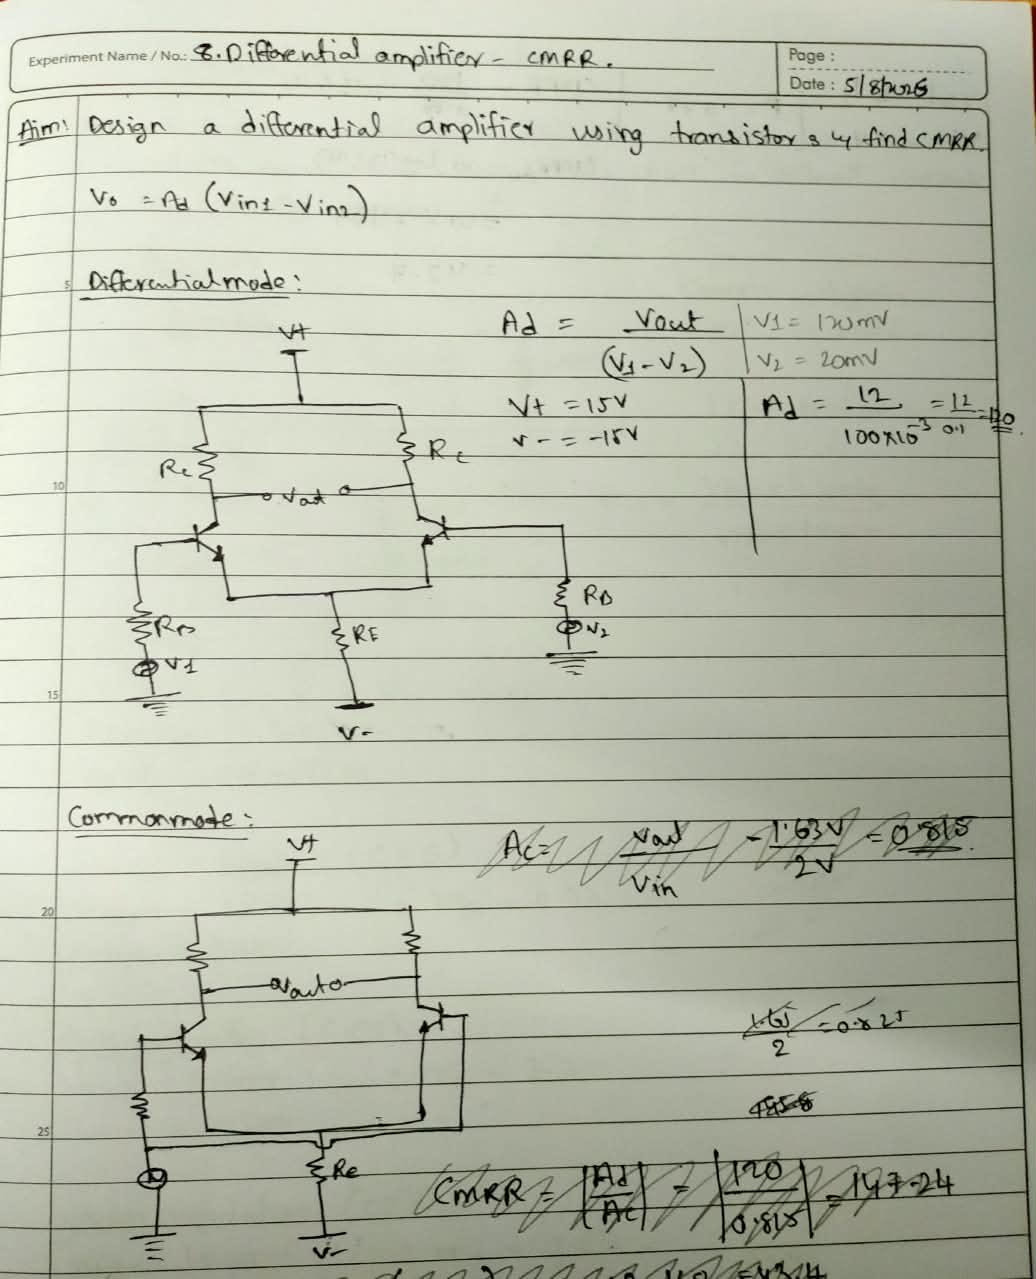
\includegraphics[width=0.85\textwidth]{observation1.jpeg}
    \caption{Lab Notes - Page 1}
\end{figure}

\begin{figure}[H]
    \centering
    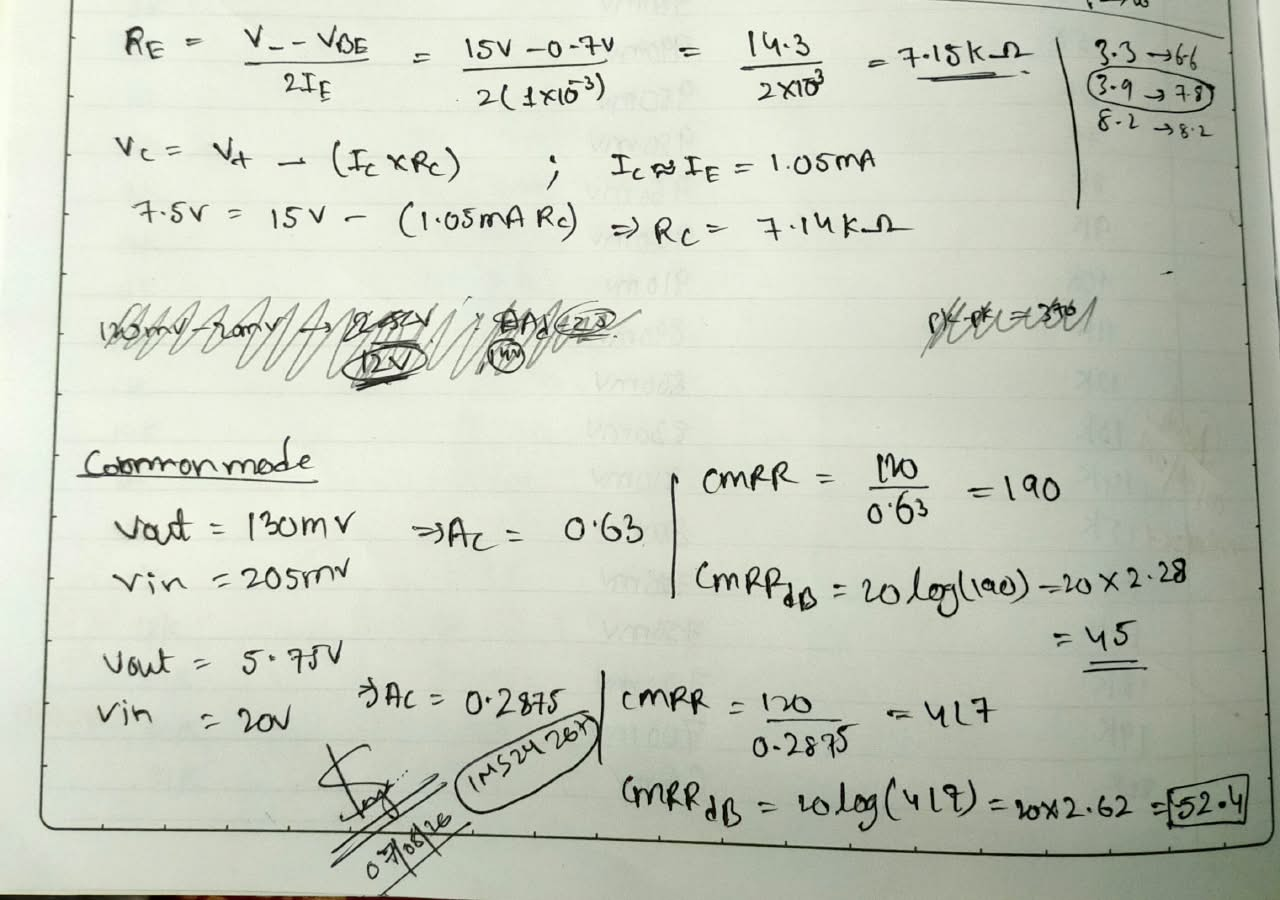
\includegraphics[width=0.85\textwidth]{observation2.jpeg}
    \caption{Lab Notes - Page 2}
\end{figure}

\end{document}
